\section{РАЗРАБОТКА ПРОГРАММНОГО ПРОДУКТА}

\subsection{Высокоуровневая архитектура}

Подводка к архитектуре.
На рисунке ~\ref{neuro_model} представлена общая арихетктура продукта.

\begin{figure}
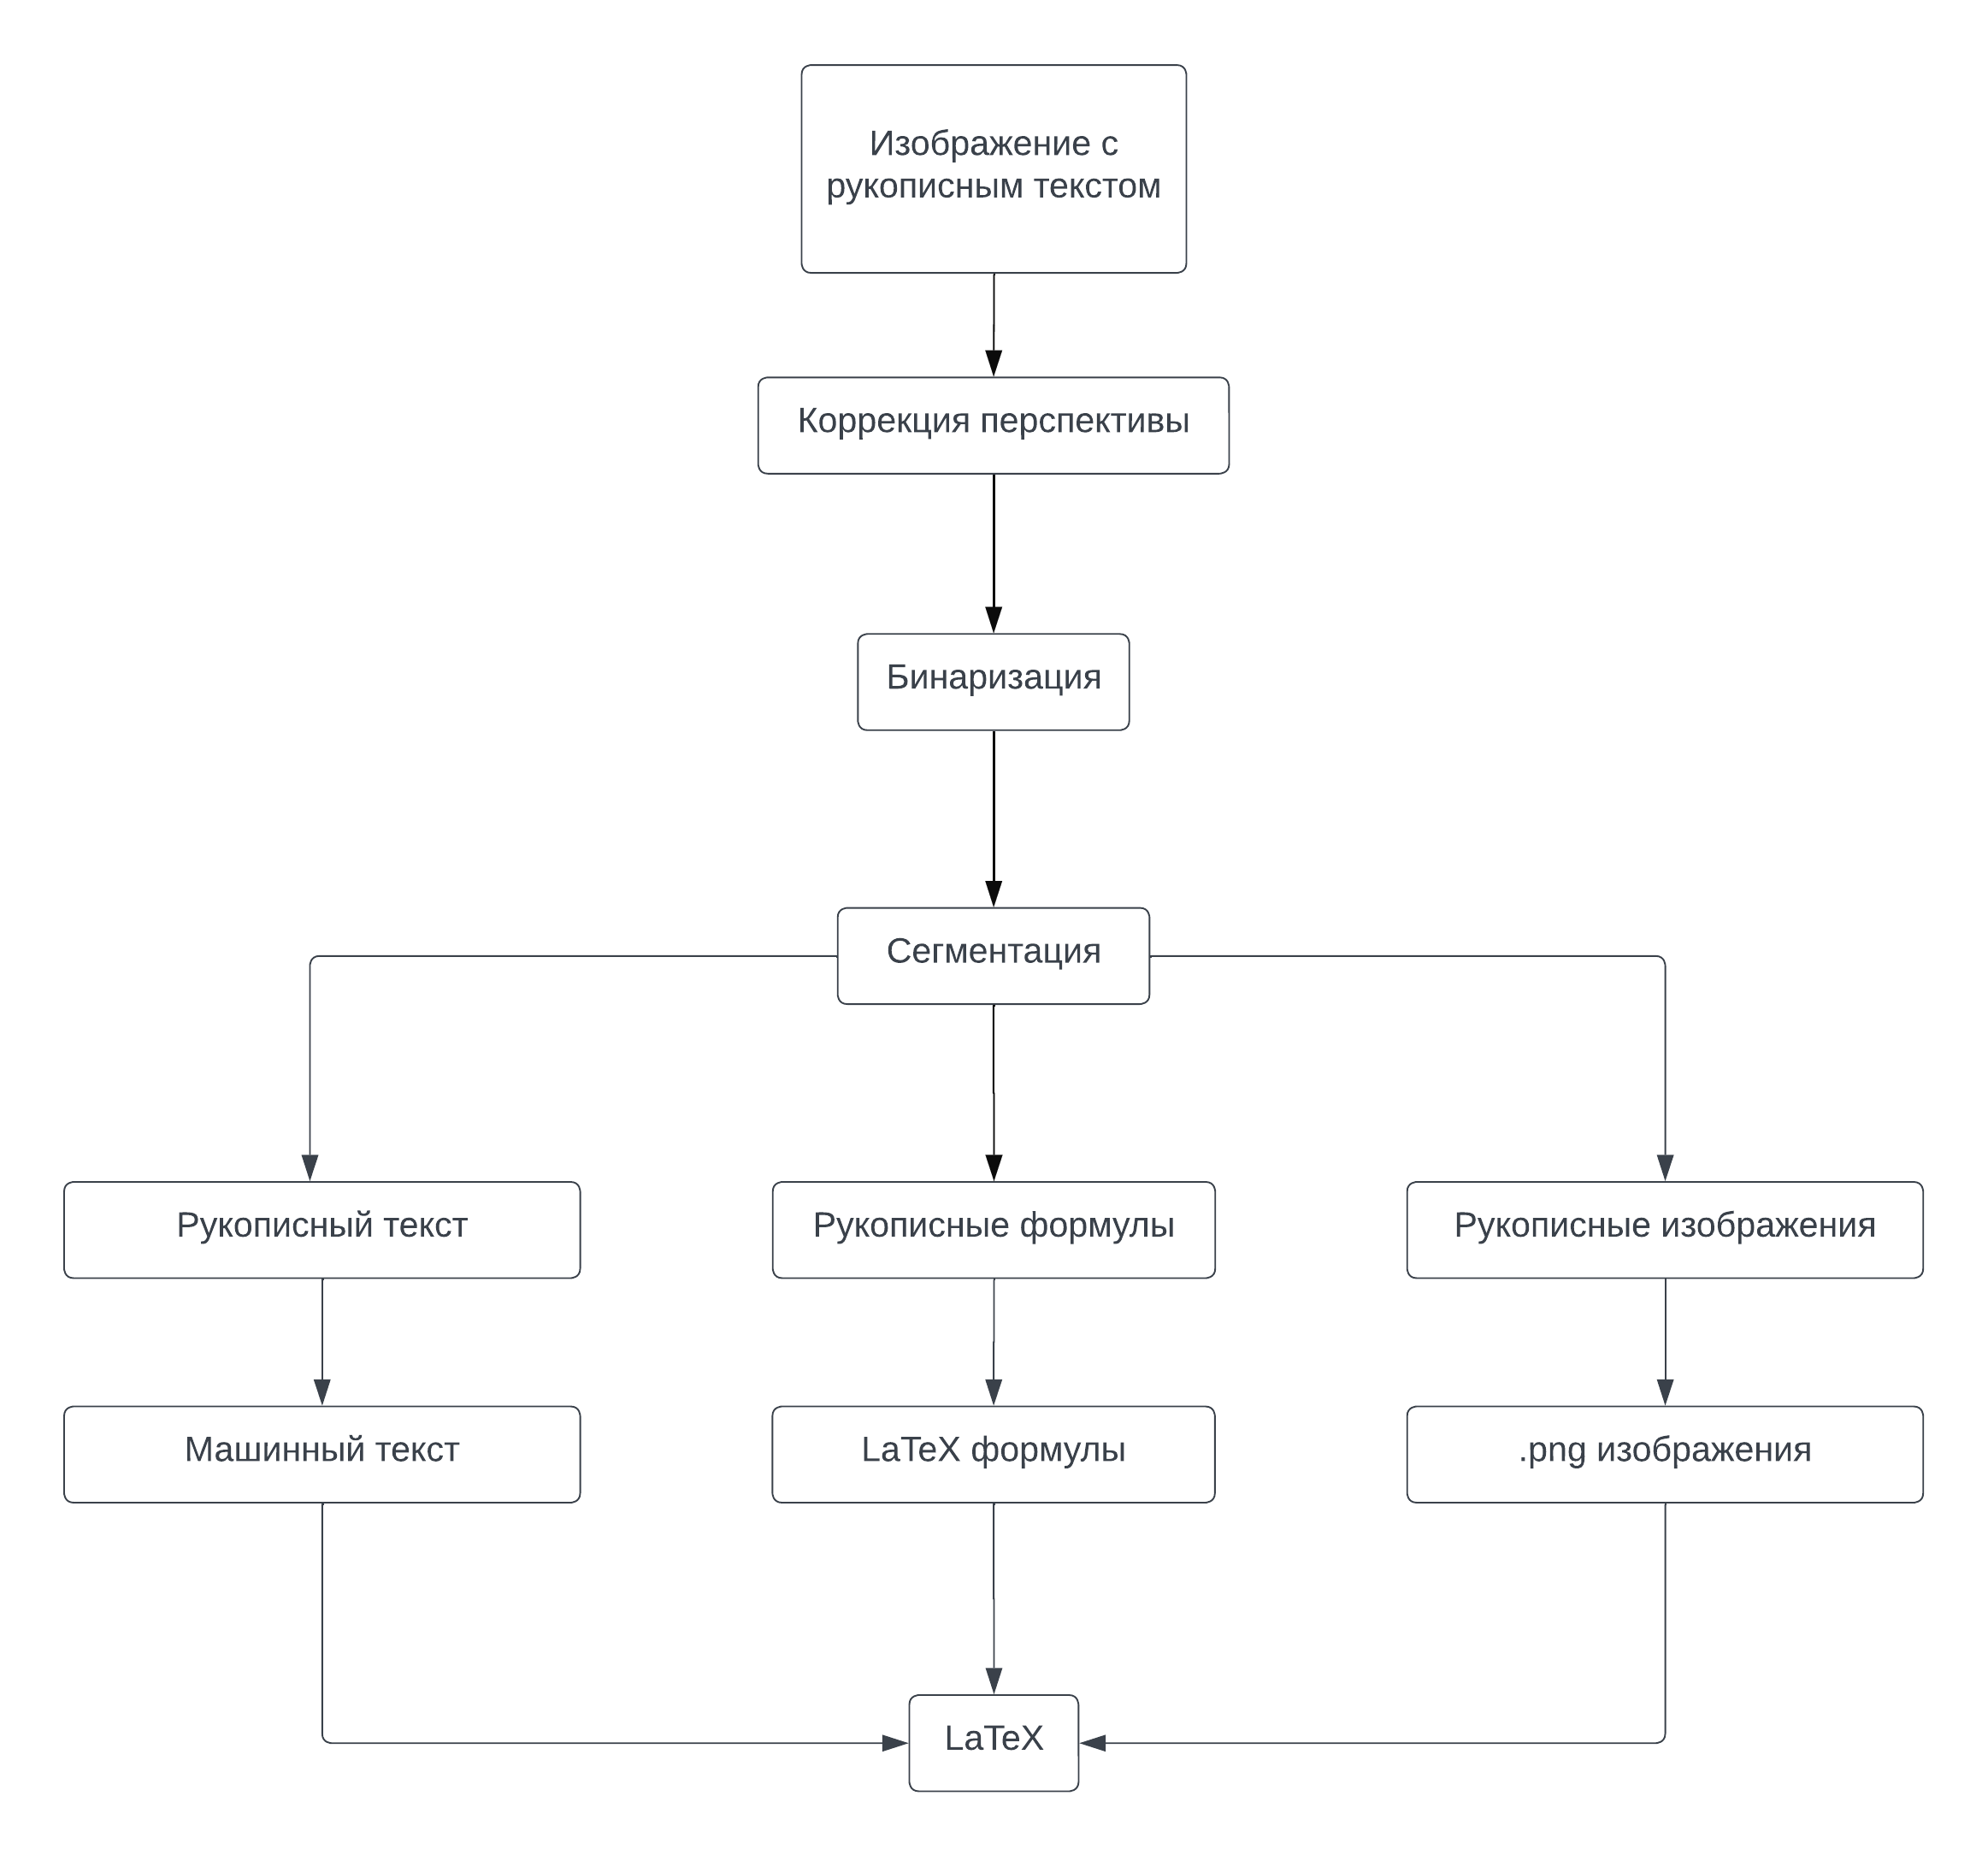
\includegraphics[scale=0.75]{img/Blank_diagram.png}
\caption{Общая архитектура модели}
\label{neuro_model}
\end{figure}

Коррекция перспективы необходима для устранения шума на изображении и получения лучшего результата. Она состоит из нескольких этапов, представленных на рисунке ~\ref{perspective_correction}. 
Также на рисунке представлены результаты, получаемые на каждом из этапов обработки.

\begin{figure}
    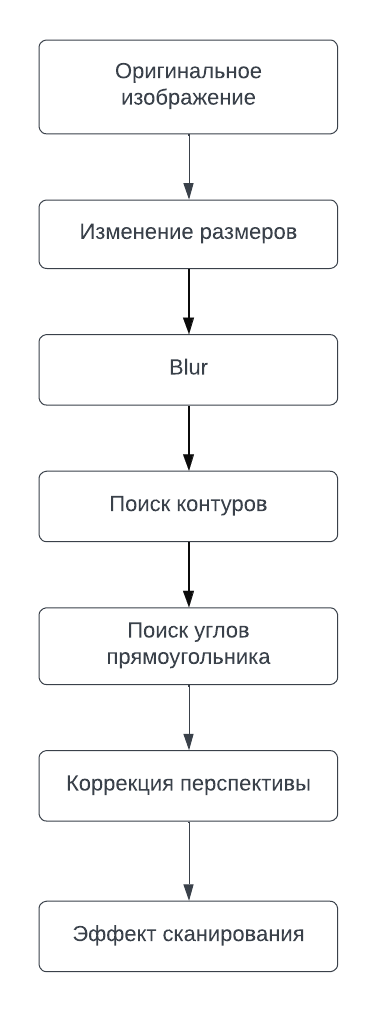
\includegraphics[scale=0.75]{img/perspective_correction}
    \caption{Этапы коррекции перспективы изображения}
    \label{perspective_correction}
\end{figure}

На начальном этапе мы имеем изображение, показанное на рисунке ~\ref{input}

\begin{figure}
    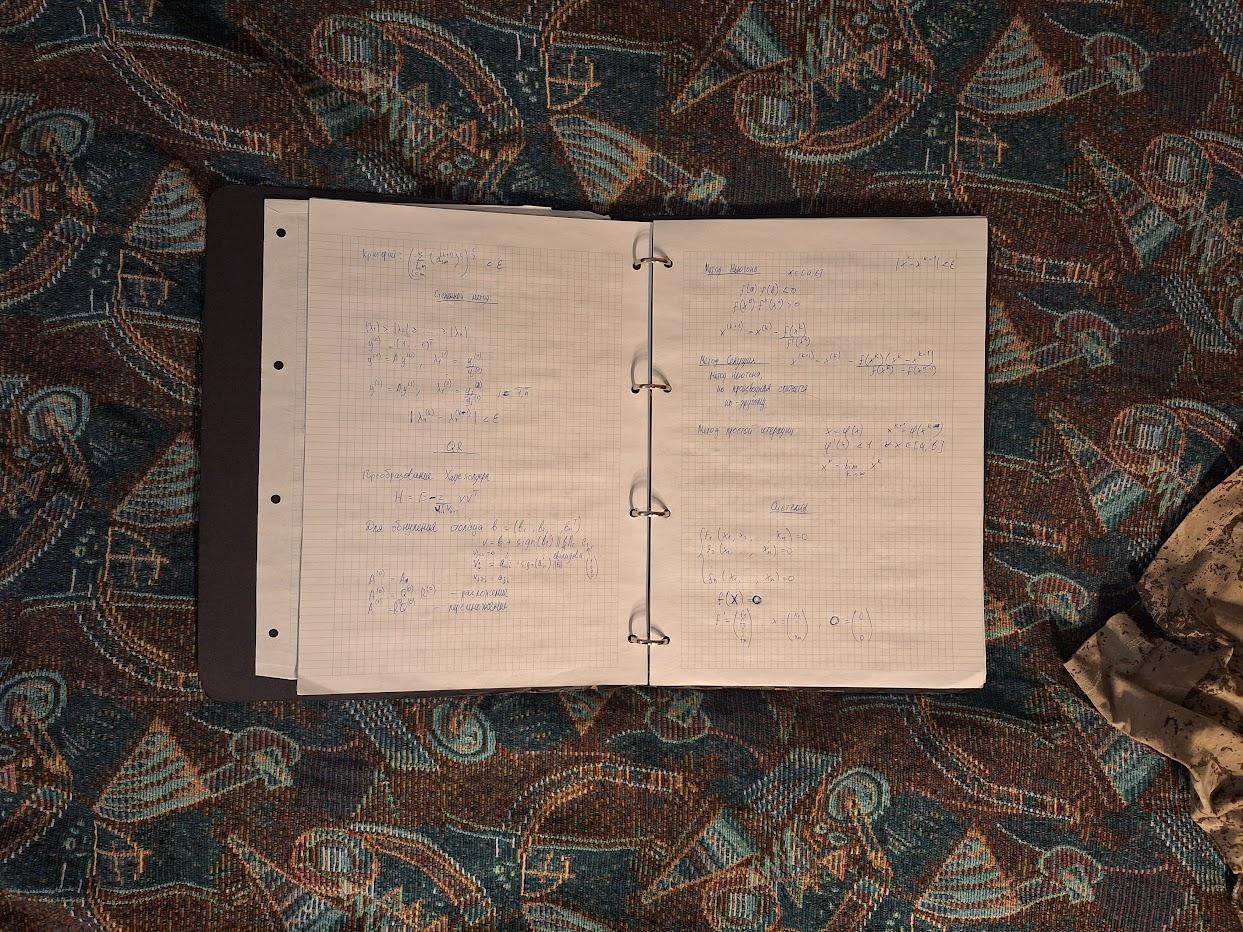
\includegraphics[scale=0.25]{img/input}
    \caption{Начальное изображение}
    \label{input}
\end{figure}

Для начала необходимо удалить текст с изображения. Для этого несколько раз производится морфологическая операция закрытия с ядром $3\times3$. 
После этого к изображению применяется алгоритм сегментации $GrabCut$ \cite{grab_cut}. На выходе данного этапа имеем изображение, представленное на рисунке ~\ref{grab_cut}

\begin{figure}
    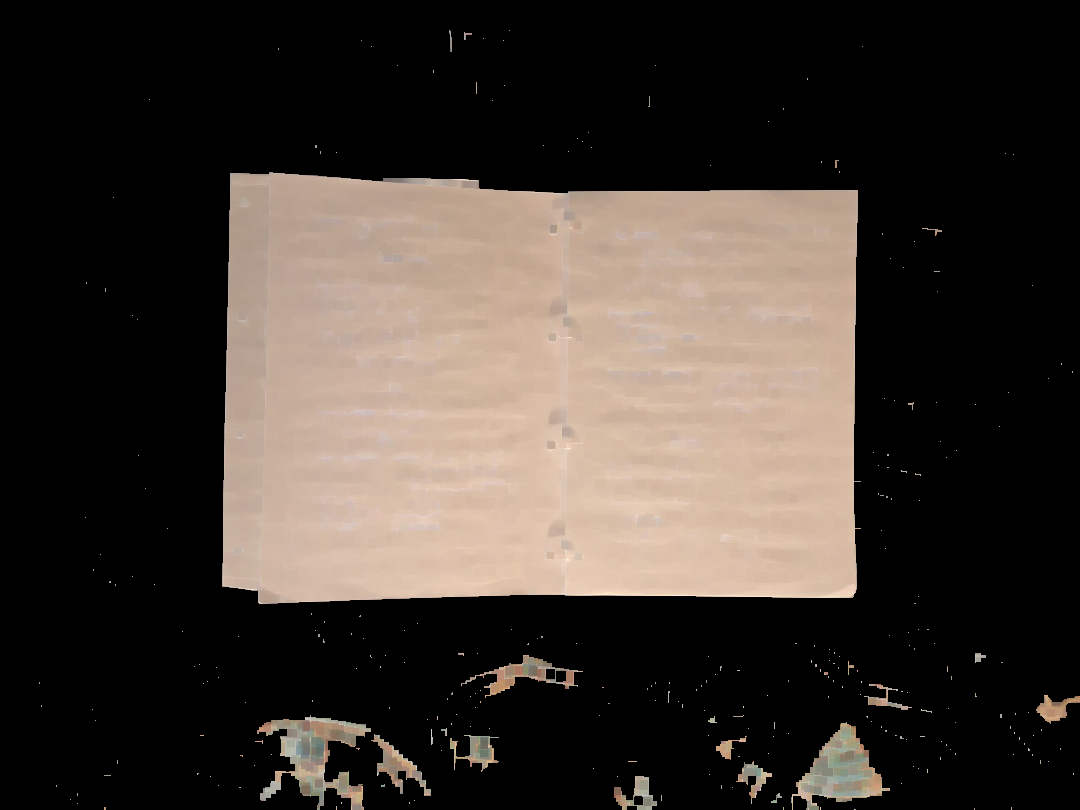
\includegraphics[scale=0.25]{img/grab_cut}
    \caption{Изображение после сегментации алгоритмом $GrabCut$}
    \label{grab_cut}
\end{figure}

На следующем этапе необходимо выделить контуры на полученном изображении. Для этого изображение переводится в серый цвет, затем к нему применяется алгоритм Гауссовского размытия \cite{gauss_blur}. После этого применяется алгоритм поиска ребер Канни \cite{canny}.
На выходе данного этапа имеем изображение, представленное на рисунке ~\ref{canny}

\begin{figure}
    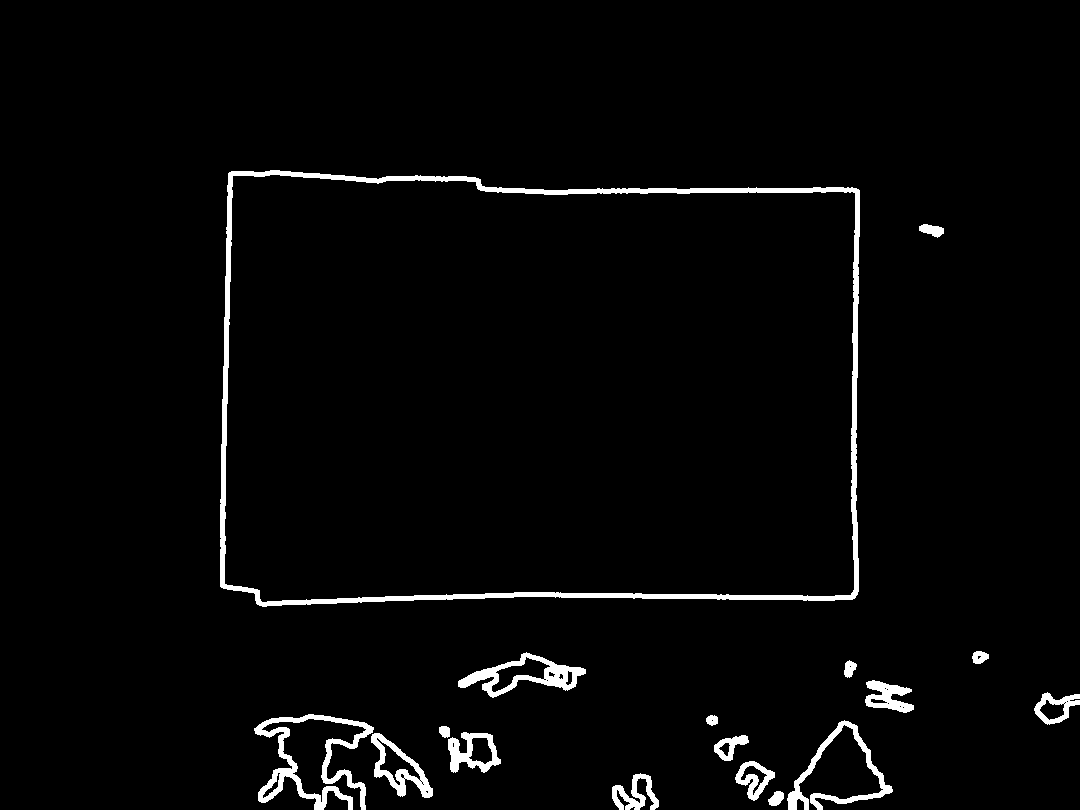
\includegraphics[scale=0.25]{img/edges}
    \caption{Ребра, найденные на изображении}
    \label{canny}
\end{figure}

На этапе нахождения контуров берутся ребра, полученные на предыдущем этапе. Находим контуры с помощью алгоритма, встроенного в $openCV$ \cite{contours}. 
Среди найденных контуров оставляем 5 контуров с наибольшей площадью. На выходе данного этапа имеем изображение, представленное на рисунке ~\ref{contours}

\begin{figure}
    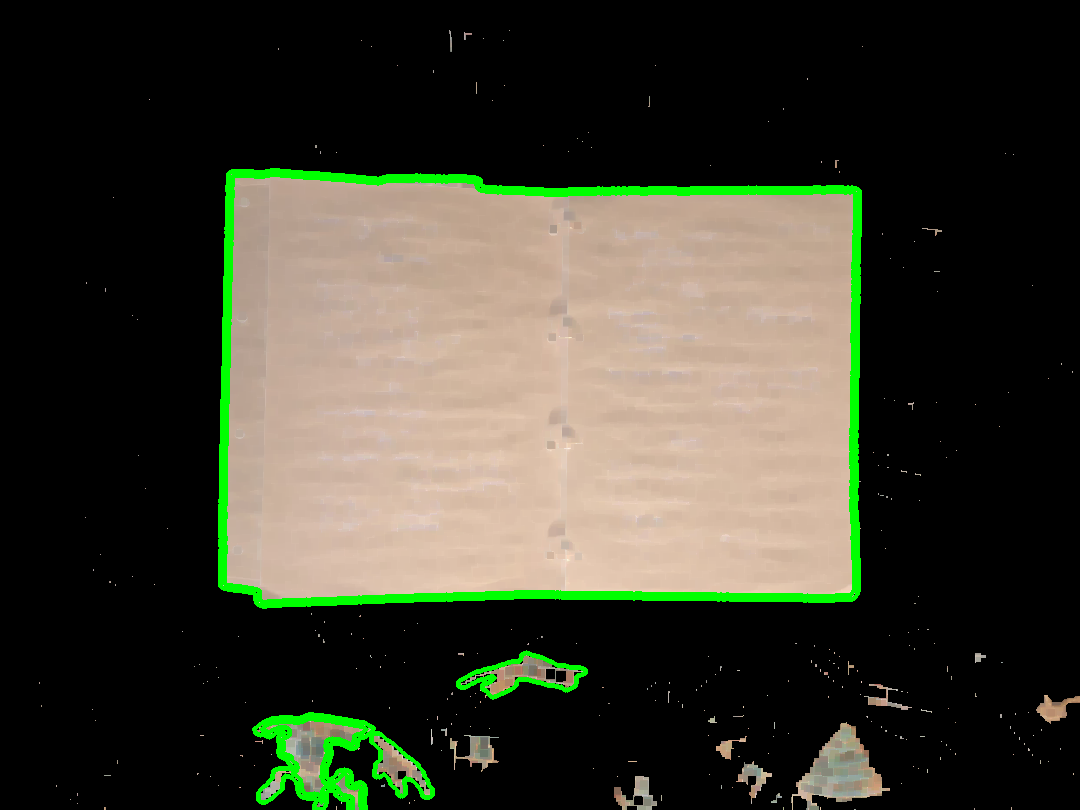
\includegraphics[scale=0.25]{img/contours}
    \caption{Найденные алгоритмом контуры}
    \label{contours}
\end{figure}

Теперь необходимо среди оставленных контуров найти координаты вершин прямоугольника (если такой есть). Для этого пытаемся аппроксимировать контур с помощью встроенной в $openCV$ \cite{opencv_approx} функции и найти прямоугольник.
После определения прямоугольника сортируем вершины в нужном порядке:
\begin{enumerate}[arabic]
    \item Левая верхняя вершина
    \item Правая нижняя вершина
    \item Правая верхняя вершина
    \item Левая нижняя вершина
\end{enumerate}

На выходе данного этапа имеем изображение, представленное на рисунке ~\ref{corners}

\begin{figure}
    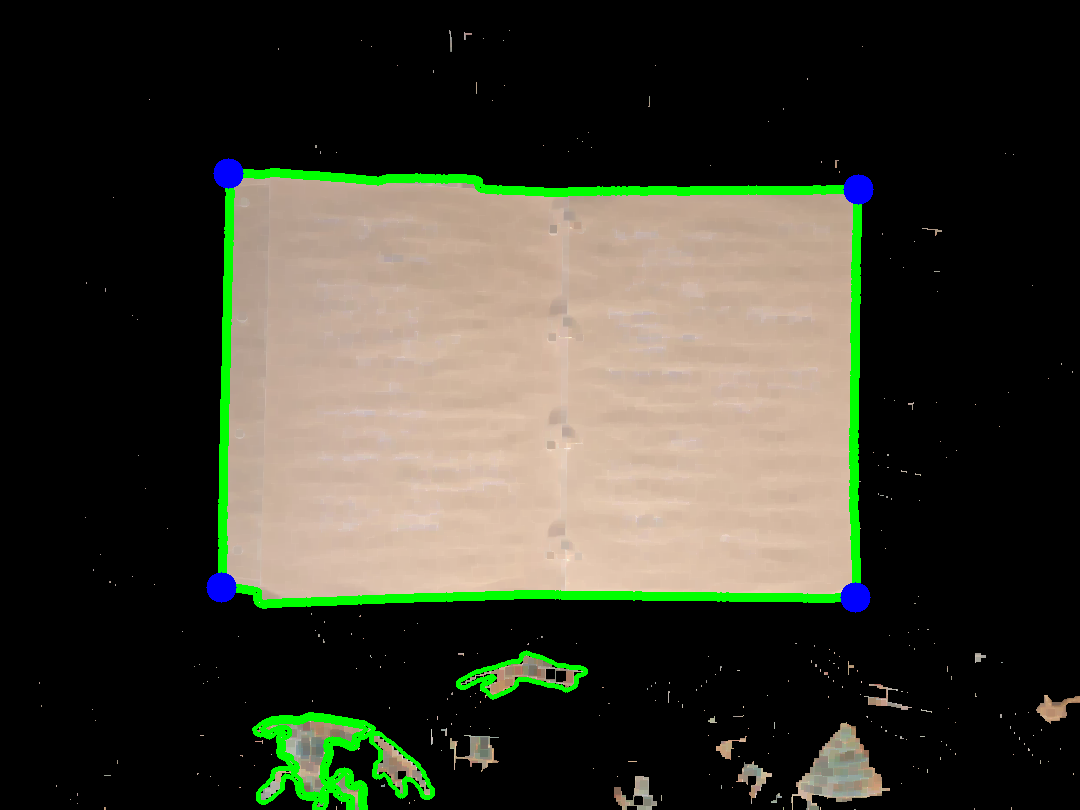
\includegraphics[scale=0.25]{img/corners}
    \caption{Найденные вершины прямоугольника}
    \label{corners}
\end{figure}

На финальном этапе по имеющимся координатам прямоугольника, представляющего лист бумаги, осуществляем коррекцию перспективы. Для этого находим матрицу коррекции \cite{opencv_perspective_transform} и примянем ее к изображению \cite{opencv_warp_perspective}.
Получаем результирующее изображение, показанное на рисунке ~\ref{perspective_correction}
\begin{figure}
    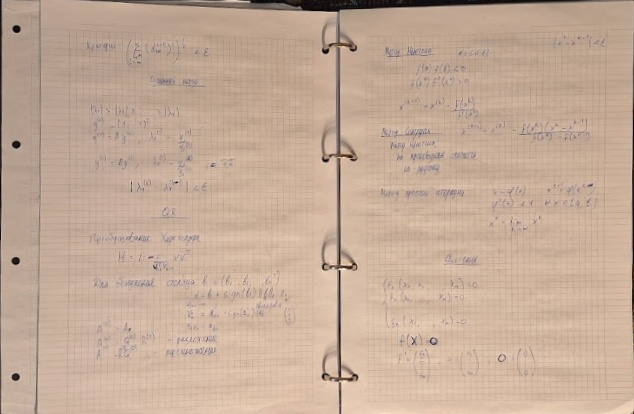
\includegraphics[scale=0.25]{img/perspective_output}
    \caption{Результирующее изображение}
    \label{perspective_correction}
\end{figure}